\subsection{Présentation}
L'application se présente comme un système d'exploitation mobile simplifié fonctionnant grâce à quelques modules de base comme le core, l'interface graphique, un émulateur, tous étant remplaceables très facilement car ce sont en réalité des plugins branchés sur la plateforme Onyx avec plus ou moins de dépendances les uns entre les autres.

\subsection{Structure}

\subsubsection{Diagramme de classes}
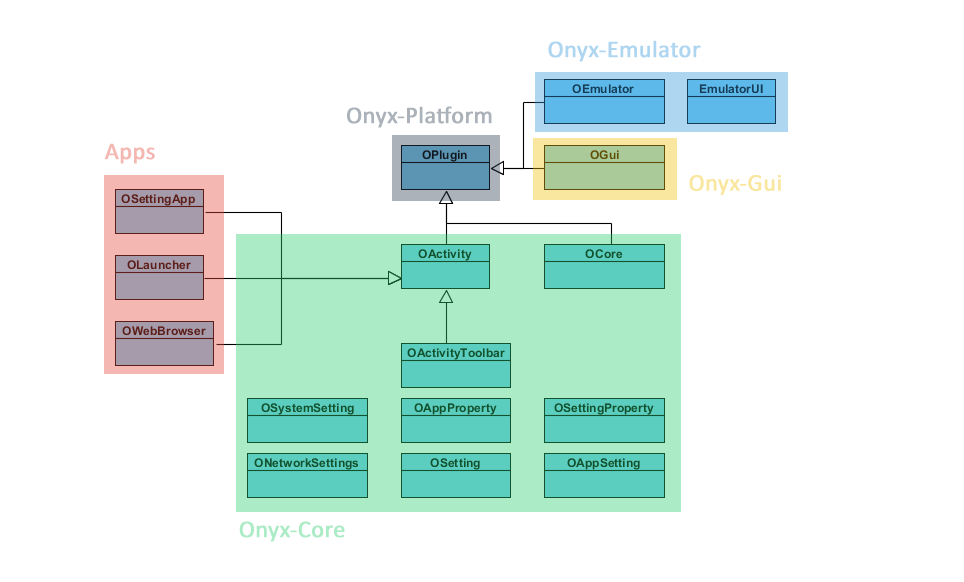
\includegraphics[width=20cm]{figures/class_diagram_app.png}

\subsection{Créer une application}

mainActivity.java

\begin{verbatim}
package com.onyx.myapppackage;
import com.onyx.core.OActivity;

public class OWebBrowser extends OActivity {
    @Override
    public void onCreate() {
        super.onCreate();
        //Some javafx code
    }
}
\end{verbatim}

OManifest

\begin{verbatim}
<?xml version="1.0"?>
<manifest>
    <id>com.onyx.myapppackage</id>
    <version>${project.version}</version>
    <name>My App Package</name>
    <description></description>

    <application>
        <mainActivity>com.onyx.myapp.mainActivity</mainActivity>
        <name>My App</name>
        <id>com.onyx.myapppackage.myapp</id>
    </application>
</manifest>
\end{verbatim}

pom.xml

<?xml version="1.0" encoding="UTF-8"?>
<project xmlns="http://maven.apache.org/POM/4.0.0"
         xmlns:xsi="http://www.w3.org/2001/XMLSchema-instance"
         xsi:schemaLocation="http://maven.apache.org/POM/4.0.0 http://maven.apache.org/xsd/maven-4.0.0.xsd">
    <parent>
        <artifactId>onyx</artifactId>
        <groupId>com.onyx</groupId>
        <version>1.0.0-SNAPSHOT</version>
    </parent>
    <modelVersion>4.0.0</modelVersion>

    <artifactId>onyx-app-my-app</artifactId>

    <dependencies>
        <dependency>
            <groupId>${project.groupId}</groupId>
            <artifactId>onyx-core</artifactId>
            <version>${project.version}</version>
            <scope>provided</scope>
        </dependency>
    </dependencies>
</project>